\documentclass{beamer}
\usepackage{amsmath}
\usepackage{hyperref}
\usepackage{listings}
\usepackage{xcolor}
\hypersetup{colorlinks=true, citecolor=blue, filecolor=blue, linkcolor=blue, urlcolor=blue}
\definecolor{codegreen}{rgb}{0,0.6,0}
\definecolor{codegray}{rgb}{0.5,0.5,0.5}
\definecolor{codepurple}{rgb}{0.58,0,0.82}
\definecolor{backcolour}{rgb}{0.95,0.95,0.92}
 
\lstdefinestyle{mystyle}{
    backgroundcolor=\color{backcolour},   
    commentstyle=\color{codegreen},
    keywordstyle=\color{magenta},
    numberstyle=\tiny\color{codegray},
    stringstyle=\color{codepurple},
    basicstyle=\ttfamily\footnotesize,
    breakatwhitespace=false,         
    breaklines=true,                 
    captionpos=b,                    
    keepspaces=true,                 
    %numbers=left,                    
    numbersep=5pt,                  
    showspaces=false,                
    showstringspaces=false,
    showtabs=false,                  
    tabsize=2
}
 
\lstset{style=mystyle}

\mode<presentation> {

% The Beamer class comes with a number of default slide themes
% which change the colors and layouts of slides. Below this is a list
% of all the themes, uncomment each in turn to see what they look like.

%\usetheme{default}
\usetheme{AnnArbor}
%\usetheme{Antibes}
%\usetheme{Bergen}
%\usetheme{Berkeley}
%\usetheme{Berlin}
%\usetheme{Boadilla}
%\usetheme{CambridgeUS}
%\usetheme{Copenhagen}
%\usetheme{Darmstadt}
%\usetheme{Dresden}
%\usetheme{Frankfurt}
%\usetheme{Goettingen}
%\usetheme{Hannover}
%\usetheme{Ilmenau}
%\usetheme{JuanLesPins}
%\usetheme{Luebeck}
%\usetheme{Madrid}
%\usetheme{Malmoe}
%\usetheme{Marburg}
%\usetheme{Montpellier}
%\usetheme{PaloAlto}
%\usetheme{Pittsburgh}
%\usetheme{Rochester}
%\usetheme{Singapore}
%\usetheme{Szeged}
%\usetheme{Warsaw}

% As well as themes, the Beamer class has a number of color themes
% for any slide theme. Uncomment each of these in turn to see how it
% changes the colors of your current slide theme.

%\usecolortheme{albatross}
%\usecolortheme{beaver}
%\usecolortheme{beetle}
%\usecolortheme{crane}
%\usecolortheme{dolphin}
%\usecolortheme{dove}
%\usecolortheme{fly}
%\usecolortheme{lily}
%\usecolortheme{orchid}
%\usecolortheme{rose}
%\usecolortheme{seagull}
%\usecolortheme{seahorse}
%\usecolortheme{whale}
%\usecolortheme{wolverine}

%\setbeamertemplate{footline} % To remove the footer line in all slides uncomment this line
\setbeamertemplate{footline}[page number] % To replace the footer line in all slides with a simple slide count uncomment this line

\setbeamertemplate{navigation symbols}{} % To remove the navigation symbols from the bottom of all slides uncomment this line
}

\usepackage{graphicx} % Allows including images
\usepackage{booktabs} % Allows the use of \toprule, \midrule and \bottomrule in tables
%\usepackage {tikz}
\usepackage{tkz-graph}
\GraphInit[vstyle = Shade]
\tikzset{
  LabelStyle/.style = { rectangle, rounded corners, draw,
                        minimum width = 2em, fill = yellow!50,
                        text = red, font = \bfseries },
  VertexStyle/.append style = { inner sep=5pt,
                                font = \normalsize\bfseries},
  EdgeStyle/.append style = {->, bend left} }
\usetikzlibrary {positioning}
%\usepackage {xcolor}
\definecolor {processblue}{cmyk}{0.96,0,0,0}
%----------------------------------------------------------------------------------------
%	TITLE PAGE
%----------------------------------------------------------------------------------------

\title[Optimization]{Numerical Optimization 03: Bracket and Zoom} % The short title appears at the bottom of every slide, the full title is only on the title page

\author{Qiang Zhu} % Your name
\institute[University of Nevada Las Vegas] % Your institution as it will appear on the bottom of every slide, may be shorthand to save space
{
University of Nevada Las Vegas\\ % Your institution for the title page
\medskip
}
\date{\today} % Date, can be changed to a custom date

\begin{document}

\begin{frame}
\titlepage % Print the title page as the first slide
\end{frame}

\begin{frame}
\frametitle{Overview} % Table of contents slide, comment this block out to remove it
\tableofcontents % Throughout your presentation, if you choose to use \section{} and \subsection{} commands, these will automatically be printed on this slide as an overview of your presentation
\end{frame}

%----------------------------------------------------------------------------------------
%	PRESENTATION SLIDES
%----------------------------------------------------------------------------------------

%------------------------------------------------

\section{Bracketing Methods}
\begin{frame}{Bracketing}
\begin{itemize}
    \item identifying an interval in which a local minimum lies and then successively shrinking the interval.
    \item applied to a unimodal function
\end{itemize}
A \textcolor{blue}{unimodal function} $f$ is one where there is a unique $x_0$, such that $f$ is monotonically decreasing for $x \leq x_0$ and monotonically increasing for $x \geq x_0$. It follows from this definition that the unique global minimum is at $x_0$, and there are no other local minima.
\begin{figure}
\centering
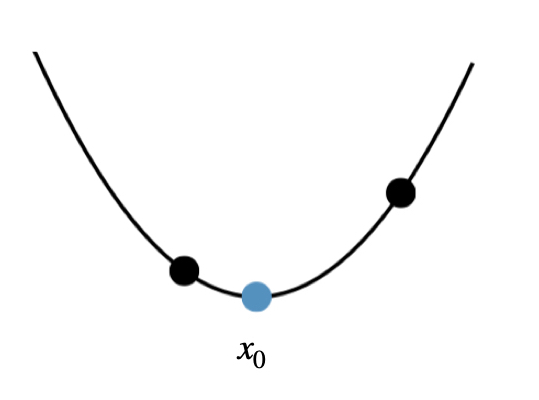
\includegraphics[width=60mm]{Figs/unimodal.jpeg}
\end{figure}
\end{frame}

%\section{Finding an Initial Bracket}
\begin{frame}{Initial Bracket}
When optimizing a function, we often start by first bracketing an interval containing a local minimum.
\begin{itemize}
    \item Starting at a given point, a trial move in the positive direction (1e-2) 
    \item search in the downhill direction to find a new point that exceeds the lowest point. 
    \item expand the step size by some factor of 2. 
\end{itemize}
\begin{figure}
\centering
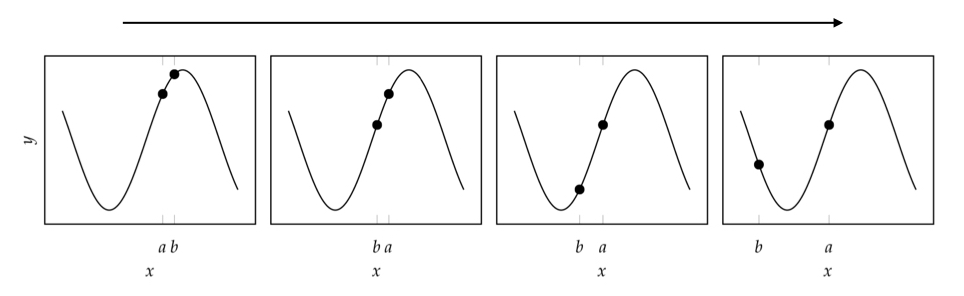
\includegraphics[width=120mm]{Figs/bracket.jpeg}
\end{figure}
\end{frame}


\section{Fibonacci Search}
\begin{frame}{Fibonacci Search}
\begin{columns}
\begin{column}{.6\textwidth}
Suppose we have a unimodal $f$ bracketed by the interval $[a, b]$.
\begin{itemize}
    \item Query $f$ on the 1/3 and 2/3 points on the interval
    \item Query $f$ on the center of the new interval
    \item Three queries ensures to shrink the interval by a factor of three
    \item $\cdots$
\end{itemize}
   
This actually follows %a \textcolor{red}{Fibonacci sequence}!
\begin{equation*}
F_n = 
    \begin{cases}
    1 & \textrm{if~} n\leq 2\\
    F_{n-1} + F_{n-2} & \textrm{otherwise}
    \end{cases}
\end{equation*}

\end{column}

\begin{column}{.4\textwidth}
\end{column}

\end{columns}
\end{frame}

\begin{frame}{Fibonacci Search Algorithm}
Let's try to formulate the problem in a more rigorous way. 
Ideally, we want to shrink the interval $[a, b]$ within $n$ iterations. For each update, we want to shrink by a factor of $\tau$,
\begin{columns}

\begin{column}{0.6 \textwidth}
\begin{equation*}
   b_{k+1} - a_{k+1} = \frac{F_{n-k}}{F_{n-k+1}}(b_k - a_k)
\end{equation*}
\begin{equation*}
\begin{split}
    F_0 &= F_1 = 1,\\
    F_{k+1} &= F_k + F_{k-1}~~~~~(k=1, 2, \cdots),     
\end{split}
\end{equation*}
Therefore,
\begin{equation*}
\begin{split}
    b_n - a_n &= \frac{F_1}{F_2}(b_{n-1}- a_{n-1})\\
              &= \frac{F_1}{F_2}\frac{F_2}{F_3} \cdots \frac{F_{n-1}}{F_n} (b_1-a_1)\\
              &= \frac{1}{F_n}(b_1 - a_1)
              %= \frac{1}{r^n}(b_1 - a_1)
\end{split}
\end{equation*}
\end{column}

\begin{column}{0.4 \textwidth}
\centering
\textcolor{blue}{Solution of $F_k$}\\
let $F_k = \tau^k$
\begin{equation*}
    \tau^2 = \tau + 1
\end{equation*}
\begin{equation*}
\begin{split}
    \tau_{1,2} &= \frac{1\pm \sqrt{5}}{2}\\
    F_k & = A\tau_1^k + B\tau_2^k
\end{split}
\end{equation*}

Since $F_0 = F_1 = 1$, 
\begin{equation*}
    F_k = \frac{1}{\sqrt{5}} (\tau_1^{k+1} - \tau_2^{k+1})
\end{equation*}
\end{column}

\end{columns}

\end{frame}

%\end{frame}

\begin{frame}{Fibonacci Algorithm}
Suppose we have a unimodal $f$ bracketed by the interval [a, b].
\begin{enumerate}
    \item Query $f$ on two points ($\lambda_k, \mu_k$) on the interval $[a_k, b_k]$
    \begin{equation*}
    \begin{split}
        \lambda_k &= a_k + \bigg(1-\frac{F_{n-k}}{F_{n-k+1}}\bigg)(b_k - a_k)\\
        \mu_k &= a_k + \frac{F_{n-k}}{F_{n-k+1}}(b_k - a_k)        
    \end{split}
    \end{equation*}
    \item if $f(\lambda_k) > f(\mu_k)$, go to step 3; otherwise, go to step 4
    \item if $b_k - \lambda_k < \delta$, terminate. otherwise
    \begin{equation*}
        a_{k+1} = \lambda_k, ~~ b_{k+1} = b_k, 
    \end{equation*}
    \item if $u_k - a_k \leq \delta$, terminate. Otherwise
    \begin{equation*}
        a_{k+1} = a_k, b_{k+1} = \mu_k, ~~ \mu_{k+1} = \lambda_k, 
    \end{equation*}
    \item k += 1, go to step 2
\end{enumerate}
\end{frame}

\section{0.618 Search}

\begin{frame}{Golden Ratio Search}
If we take the limit for large $n$, the ratio between successive values of the Fibonacci sequence approaches the golden ratio:

\begin{equation*}
\lim_{n\rightarrow\infty} \frac{F_{k-1}}{F_k} = \frac{\sqrt{5}-1}{2} = 0.618
\end{equation*}

Therefore, we can always use 0.618 and 0.392 to check the two points within the updated interval.\\

Both Fibonacci and golden ratio searches have the property of linear scaling. Fibonacci is in principle the optimum search strategy for bracketing a unimodal function. However, golden ratio is more popular due to its simplicity.

\end{frame}

\begin{frame}{Comparison}

\begin{figure}
\centering
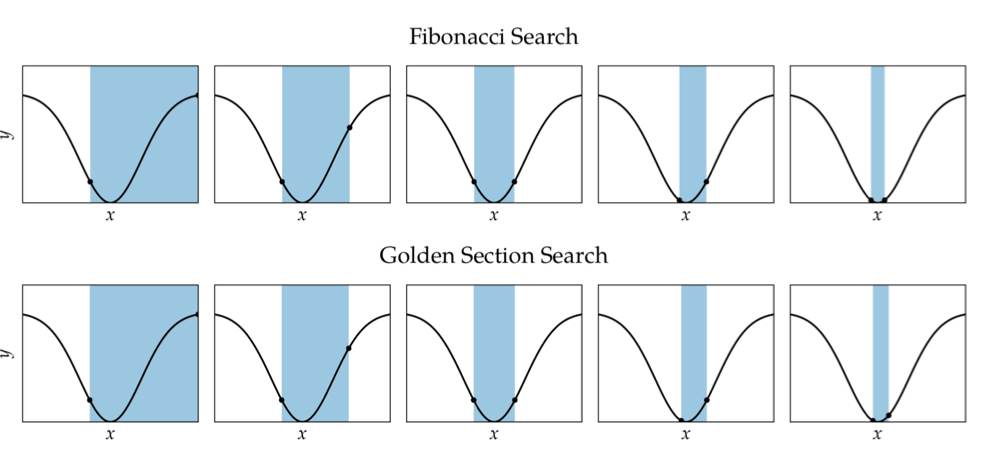
\includegraphics[width=120mm]{Figs/search.jpeg}
\end{figure}

\textcolor{blue}{Homework: reproduce the above figure by yourself!}
\end{frame}

\section{Interpolation}

\begin{frame}{Interpolation with the help of gradient}
Both Fibonacci and 0.618 searches do not need the gradient information. However, if the gradient is available, identifying the phase can be even faster. The idea is to approximate the target function in a analytic manner. 
\begin{itemize}
    \item Linear: bisection
    \item quadratic fit
    \item cubic interpolation
\end{itemize}

\end{frame}

\begin{frame}{Bisection}
The bisection method maintains a bracket $[a, b]$ in which at least one root is known to exist. If $f$ is continuous on $[a, b]$, and there is some $y \in [ f (a), f (b)]$, then the intermediate value theorem stipulates that there exists at least one $x \in [a, b]$, such that $f(x) = y$. It follows that a bracket [a, b] is guaranteed to contain a zero if $f(a)$ and $f(b)$ have opposite signs.

\begin{itemize}
    \item Starting at [$a_1, b_1]$ 
    \item if $f`(a_k) \leq 0$ and $f`(b_k) \geq 0$, let $c_k = \frac{1}{2} (a_k + b_k)$
    \item if $f`(c_k) \geq 0$, let $a_{k+1} = a_k$, $b_{k+1}=c_k$, otherwise, $a_{k+1}=c_k$, $b_{k+1}=b_k$ 
    \item terminate if $(b_{k+1} - a_{k+1}) \leq \delta $ or it reaches the given number of iterations
\end{itemize}

Bisection method is commonly used to find roots of a function, or points where the function is zero.    
\end{frame}

\begin{frame}{Quadratic fit search}
Given the bracketing point $a<b<c$, we want to find the coefficient $p_1, p_2, p_3$ which satisfies:
\begin{equation*}
    q(x) = p_1 + p_2x + p_3x^2
\end{equation*}
\begin{columns}
\begin{column}{.4\textwidth}
\begin{equation*}
    \begin{split}
        y_a &= p_1 + p_2a + p_3a^2\\
        y_b &= p_1 + p_2b + p_3b^2\\
        y_c &= p_1 + p_2c + p_3c^2
    \end{split}
\end{equation*}
\end{column}

\begin{column}{.6\textwidth}
In matrix form, we have \\
\begin{equation*}
\begin{bmatrix}
y_a\\
y_b\\
y_c
\end{bmatrix}
= 
\begin{bmatrix}
1 & a & a^2\\
1 & b & b^2\\
1 & c & c^2
\end{bmatrix}
\cdot
\begin{bmatrix}
p_1\\
p_2\\
p_3
\end{bmatrix}
\end{equation*}

\end{column}
\end{columns}

\begin{equation*}
    q(x) = y_a\frac{(x-b)(x-c)}{(a-b)(a-c)} + y_b\frac{(x-a)(x-c)}{(b-a)(b-c)} + y_c\frac{(x-a)(x-b)}{(c-a)(c-b)} 
\end{equation*}

We can solve the minimum by finding the derivative is zero:
\begin{equation*}
    x^* = \frac{1}{2} \frac{y_a(b^2-c^2) + y_b(c^2-a^2) + y_c(a^2-b^2)}{y_a(b-c) + y_b(c-a) + y_c(c-b)}
\end{equation*}
\end{frame}




\section{Summary}
\begin{frame}{Summary}
    \begin{itemize}
        \item Many optimization methods shrink a bracketing interval
        \item The step length is then selected by a zoom phase
        \item Fibonacci search and golden section search has the linear scaling of $\tau = 0.618$. They are derivative free.
        \item Root-finding methods like the bisection method can be used to find where the derivative of a function is zero.
        \item quadratic or cubic fit is more common choice in the zoom phase of line search
    \end{itemize}
\end{frame}
\end{document}

